\documentclass{beamer}\usepackage[]{graphicx}\usepackage[]{color}
%% maxwidth is the original width if it is less than linewidth
%% otherwise use linewidth (to make sure the graphics do not exceed the margin)
\makeatletter
\def\maxwidth{ %
  \ifdim\Gin@nat@width>\linewidth
    \linewidth
  \else
    \Gin@nat@width
  \fi
}
\makeatother

\definecolor{fgcolor}{rgb}{0.345, 0.345, 0.345}
\newcommand{\hlnum}[1]{\textcolor[rgb]{0.686,0.059,0.569}{#1}}%
\newcommand{\hlstr}[1]{\textcolor[rgb]{0.192,0.494,0.8}{#1}}%
\newcommand{\hlcom}[1]{\textcolor[rgb]{0.678,0.584,0.686}{\textit{#1}}}%
\newcommand{\hlopt}[1]{\textcolor[rgb]{0,0,0}{#1}}%
\newcommand{\hlstd}[1]{\textcolor[rgb]{0.345,0.345,0.345}{#1}}%
\newcommand{\hlkwa}[1]{\textcolor[rgb]{0.161,0.373,0.58}{\textbf{#1}}}%
\newcommand{\hlkwb}[1]{\textcolor[rgb]{0.69,0.353,0.396}{#1}}%
\newcommand{\hlkwc}[1]{\textcolor[rgb]{0.333,0.667,0.333}{#1}}%
\newcommand{\hlkwd}[1]{\textcolor[rgb]{0.737,0.353,0.396}{\textbf{#1}}}%
\let\hlipl\hlkwb

\usepackage{framed}
\makeatletter
\newenvironment{kframe}{%
 \def\at@end@of@kframe{}%
 \ifinner\ifhmode%
  \def\at@end@of@kframe{\end{minipage}}%
  \begin{minipage}{\columnwidth}%
 \fi\fi%
 \def\FrameCommand##1{\hskip\@totalleftmargin \hskip-\fboxsep
 \colorbox{shadecolor}{##1}\hskip-\fboxsep
     % There is no \\@totalrightmargin, so:
     \hskip-\linewidth \hskip-\@totalleftmargin \hskip\columnwidth}%
 \MakeFramed {\advance\hsize-\width
   \@totalleftmargin\z@ \linewidth\hsize
   \@setminipage}}%
 {\par\unskip\endMakeFramed%
 \at@end@of@kframe}
\makeatother

\definecolor{shadecolor}{rgb}{.97, .97, .97}
\definecolor{messagecolor}{rgb}{0, 0, 0}
\definecolor{warningcolor}{rgb}{1, 0, 1}
\definecolor{errorcolor}{rgb}{1, 0, 0}
\newenvironment{knitrout}{}{} % an empty environment to be redefined in TeX

\usepackage{alltt}
\IfFileExists{upquote.sty}{\usepackage{upquote}}{}
\begin{document}

\title{Wordcloud of negative and positive words}
\author{Jerrin Joe Varghese}

\begin{frame}
  \titlepage
\end{frame}

\begin{frame}
  \frametitle{Table of Contents}
    \tableofcontents
\end{frame}

\section{Install and Load libraries}
\begin{frame}[fragile]
  \frametitle{Install and Load libraries}
    \begin{itemize}
    
      \item<1->
\begin{knitrout}
\definecolor{shadecolor}{rgb}{0.969, 0.969, 0.969}\color{fgcolor}\begin{kframe}
\begin{alltt}
  \hlkwd{library}\hlstd{(dplyr)}
\end{alltt}
\end{kframe}
\end{knitrout}
      \item<2->
\begin{knitrout}
\definecolor{shadecolor}{rgb}{0.969, 0.969, 0.969}\color{fgcolor}\begin{kframe}
\begin{alltt}
  \hlkwd{library}\hlstd{(gutenbergr)}
\end{alltt}
\end{kframe}
\end{knitrout}
     \item<3->
\begin{knitrout}
\definecolor{shadecolor}{rgb}{0.969, 0.969, 0.969}\color{fgcolor}\begin{kframe}
\begin{alltt}
  \hlkwd{library}\hlstd{(tidytext)}
\end{alltt}
\end{kframe}
\end{knitrout}
    \item<4->
\begin{knitrout}
\definecolor{shadecolor}{rgb}{0.969, 0.969, 0.969}\color{fgcolor}\begin{kframe}
\begin{alltt}
  \hlkwd{library}\hlstd{(ggplot2)}
\end{alltt}
\end{kframe}
\end{knitrout}

    \item<5->
\begin{knitrout}
\definecolor{shadecolor}{rgb}{0.969, 0.969, 0.969}\color{fgcolor}\begin{kframe}
\begin{alltt}
  \hlkwd{library}\hlstd{(stringr)}
\end{alltt}
\end{kframe}
\end{knitrout}

    \item<6->
\begin{knitrout}
\definecolor{shadecolor}{rgb}{0.969, 0.969, 0.969}\color{fgcolor}\begin{kframe}
\begin{alltt}
  \hlkwd{library}\hlstd{(wordcloud)}
\end{alltt}
\end{kframe}
\end{knitrout}

    \item<7->
\begin{knitrout}
\definecolor{shadecolor}{rgb}{0.969, 0.969, 0.969}\color{fgcolor}\begin{kframe}
\begin{alltt}
  \hlkwd{library}\hlstd{(wordcloud2)}
\end{alltt}
\end{kframe}
\end{knitrout}
    \end{itemize}
   
\end{frame}

\section{Hands on Project Gutenberg}
\begin{frame}[fragile]
  \frametitle{Acess Project Gutenberg}
\begin{knitrout}
\definecolor{shadecolor}{rgb}{0.969, 0.969, 0.969}\color{fgcolor}\begin{kframe}
\begin{alltt}
  \hlstd{df}\hlkwb{<-}\hlkwd{gutenberg_works}\hlstd{(}\hlkwd{str_detect}\hlstd{(title,}\hlstr{'Dracula'}\hlstd{))}
  \hlstd{df}\hlopt{$}\hlstd{gutenberg_id}
\end{alltt}
\begin{verbatim}
## [1]   345 10150
\end{verbatim}
\begin{alltt}
  \hlstd{df}\hlopt{$}\hlstd{title}
\end{alltt}
\begin{verbatim}
## [1] "Dracula"         "Dracula's Guest"
\end{verbatim}
\end{kframe}
\end{knitrout}
\end{frame}

\section{Download Dracula the Book}
\begin{frame}[fragile]
  \frametitle{Download Dracula}
\begin{knitrout}
\definecolor{shadecolor}{rgb}{0.969, 0.969, 0.969}\color{fgcolor}\begin{kframe}
\begin{alltt}
    \hlstd{dracula}\hlkwb{<-}\hlkwd{gutenberg_download}\hlstd{(}\hlnum{345}\hlstd{)}
    \hlkwd{colnames}\hlstd{(dracula)}
\end{alltt}
\begin{verbatim}
## [1] "gutenberg_id" "text"
\end{verbatim}
\begin{alltt}
    \hlkwd{substr}\hlstd{(dracula}\hlopt{$}\hlstd{text[}\hlnum{500}\hlstd{],}\hlnum{1}\hlstd{,}\hlnum{21}\hlstd{)}
\end{alltt}
\begin{verbatim}
## [1] "my own disappointment"
\end{verbatim}
\end{kframe}
\end{knitrout}
  
\end{frame}

\section{Unpack the Words}
\begin{frame}[fragile]
  \frametitle{Unpack the Words}
\begin{knitrout}
\definecolor{shadecolor}{rgb}{0.969, 0.969, 0.969}\color{fgcolor}\begin{kframe}
\begin{alltt}
  \hlstd{dracula_words}\hlkwb{<-}\hlstd{dracula}\hlopt
    \hlkwd{unnest_tokens}\hlstd{(word,text)}
  \hlkwd{colnames}\hlstd{(dracula_words)}
\end{alltt}
\begin{verbatim}
## [1] "gutenberg_id" "word"
\end{verbatim}
\begin{alltt}
  \hlstd{dracula_words[}\hlnum{498}\hlopt{:}\hlnum{500}\hlstd{,]}
\end{alltt}
\begin{verbatim}
## # A tibble: 3 x 2
##   gutenberg_id  word
##          <int> <chr>
## 1          345  fail
## 2          345    to
## 3          345  have
\end{verbatim}
\end{kframe}
\end{knitrout}

\end{frame}


\section{The Bing Lexicon for sentiments}
\begin{frame}[fragile]
  \frametitle{The Bing Lexicon}
\begin{knitrout}
\definecolor{shadecolor}{rgb}{0.969, 0.969, 0.969}\color{fgcolor}\begin{kframe}
\begin{alltt}
  \hlstd{bing} \hlkwb{=} \hlkwd{get_sentiments}\hlstd{(}\hlstr{'bing'}\hlstd{)}
  \hlkwd{colnames}\hlstd{(bing)}
\end{alltt}
\begin{verbatim}
## [1] "word"      "sentiment"
\end{verbatim}
\begin{alltt}
  \hlstd{bing[}\hlnum{498}\hlopt{:}\hlnum{500}\hlstd{,]}
\end{alltt}
\begin{verbatim}
## # A tibble: 3 x 2
##          word sentiment
##         <chr>     <chr>
## 1     bereave  negative
## 2 bereavement  negative
## 3      bereft  negative
\end{verbatim}
\end{kframe}
\end{knitrout}
\end{frame}

\section{The Inner Join}
\begin{frame}[fragile]
  \frametitle{The Inner Join}
\begin{knitrout}
\definecolor{shadecolor}{rgb}{0.969, 0.969, 0.969}\color{fgcolor}\begin{kframe}
\begin{alltt}
  \hlstd{dracula_words} \hlkwb{<-} \hlkwd{inner_join}\hlstd{(dracula_words,bing)}
\end{alltt}


{\ttfamily\noindent\itshape\color{messagecolor}{\#\# Joining, by = "{}word"{}}}\begin{alltt}
  \hlstd{dracula_words}\hlopt{$}\hlstd{gutenberg_id} \hlkwb{<-} \hlkwa{NULL}
  \hlstd{dracula_words[}\hlnum{498}\hlopt{:}\hlnum{500}\hlstd{,]}
\end{alltt}
\begin{verbatim}
## # A tibble: 3 x 2
##      word sentiment
##     <chr>     <chr>
## 1   great  positive
## 2    love  positive
## 3 crowded  negative
\end{verbatim}
\end{kframe}
\end{knitrout}
\end{frame}

\section{Calculate Frequency for Wordcloud}
\begin{frame}[fragile]
  \frametitle{Frequency of words}
\begin{knitrout}
\definecolor{shadecolor}{rgb}{0.969, 0.969, 0.969}\color{fgcolor}\begin{kframe}
\begin{alltt}
\hlstd{dracula_words}\hlkwb{<-}\hlstd{dracula_words}\hlopt
\hlkwd{group_by}\hlstd{(word)}\hlopt
\hlkwd{summarise}\hlstd{(}\hlkwc{freq}\hlstd{=}\hlkwd{n}\hlstd{(),}\hlkwc{sentiment}\hlstd{=}\hlkwd{first}\hlstd{(sentiment))}
\hlstd{dracula_words[}\hlnum{25}\hlopt{:}\hlnum{30}\hlstd{,]}
\end{alltt}
\begin{verbatim}
## # A tibble: 6 x 3
##       word  freq sentiment
##      <chr> <int>     <chr>
## 1   aghast     1  negative
## 2    agony     8  negative
## 3    alarm     3  negative
## 4  alarmed     5  negative
## 5 alarming     1  negative
## 6    aloof     1  negative
\end{verbatim}
\end{kframe}
\end{knitrout}
\end{frame}

\section{Wordcloud}
\begin{frame}[fragile]
  \frametitle{Wordcloud}
\begin{knitrout}
\definecolor{shadecolor}{rgb}{0.969, 0.969, 0.969}\color{fgcolor}
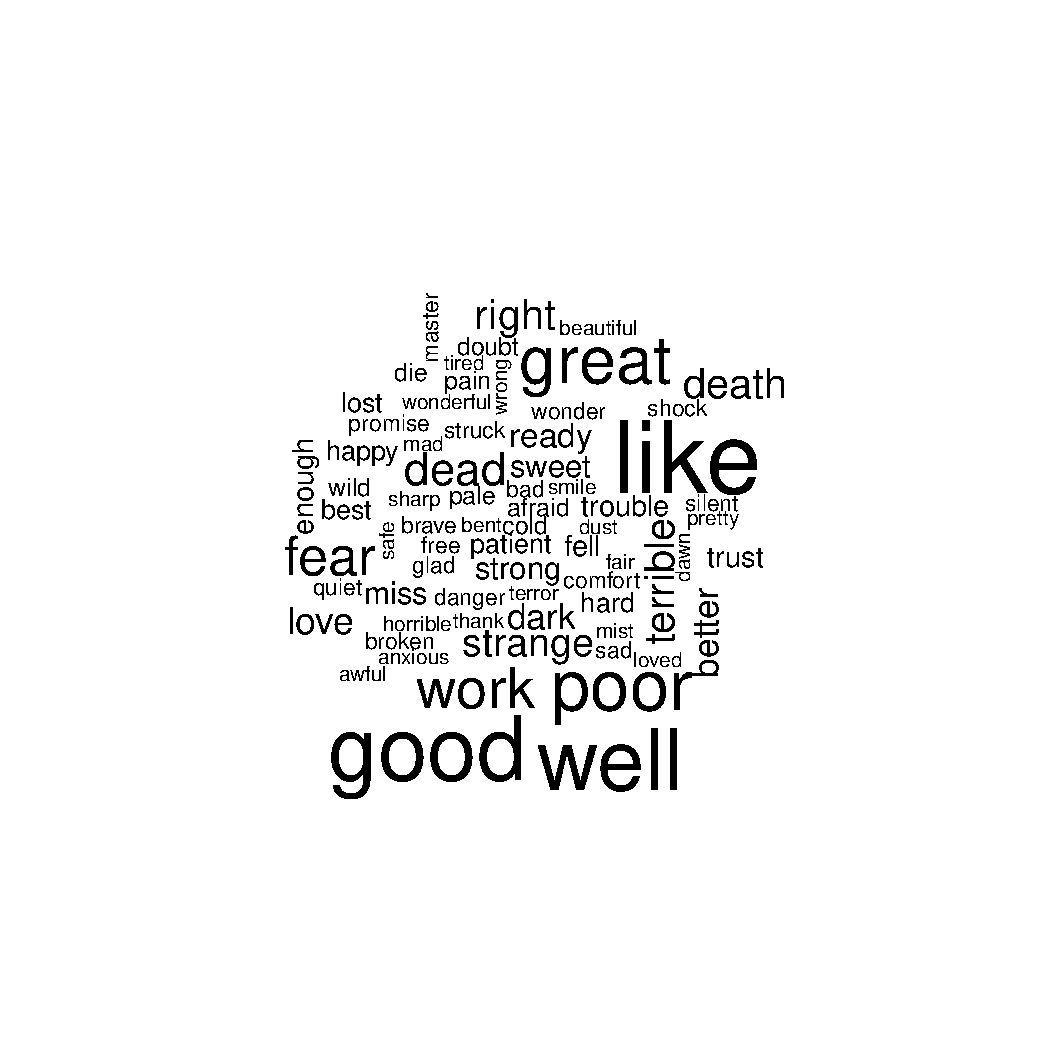
\includegraphics[width=\maxwidth]{figure/unnamed-chunk-14-1} 

\end{knitrout}

\end{frame}


\end{document}
